\documentclass[conference]{IEEEtran}
\IEEEoverridecommandlockouts

\usepackage{cite}
\usepackage{amsmath,amssymb,amsfonts}
\usepackage{algorithmic}
\usepackage{graphicx}
\usepackage{textcomp}
\usepackage{xcolor}
\usepackage[a4paper, total={184mm,239mm}]{geometry}
\def\BibTeX{{\rm B\kern-.05em{\sc i\kern-.025em b}\kern-.08em
    T\kern-.1667em\lower.7ex\hbox{E}\kern-.125emX}}

\usepackage{listings}
\usepackage{booktabs}
\usepackage{multirow}
\usepackage[normalem]{ulem}
\useunder{\uline}{\ul}{}
\usepackage{url}
\usepackage{fancyvrb}

\lstdefinestyle{Scalastyle}{
    language=scala,
    aboveskip=3mm,
    belowskip=3mm,
    showstringspaces=false,
    columns=flexible,
    basicstyle={\small\ttfamily},
    numberstyle=\tiny\color{gray},
    keywordstyle=\color{blue},
    commentstyle=\color{dkgreen},
    stringstyle=\color{mauve},
    breaklines=true,
    breakatwhitespace=true,
    tabsize=2,
    numbers=left,
    xleftmargin=2em,
    frame=single,
    framexleftmargin=1.5em,
    captionpos=b
}

\definecolor{mGreen}{rgb}{0,0.6,0}
\definecolor{mGray}{rgb}{0.5,0.5,0.5}
\definecolor{mPurple}{rgb}{0.58,0,0.82}
\definecolor{backgroundColour}{rgb}{0.95,0.95,0.92}

\lstdefinestyle{Cstyle}{
    language=C,
    aboveskip=3mm,
    belowskip=3mm,
    showstringspaces=false,
    columns=flexible,
    basicstyle={\small\ttfamily},
    numberstyle=\tiny\color{gray},
    keywordstyle=\color{blue},
    commentstyle=\color{mGreen},
    stringstyle=\color{mPurple},
    breaklines=true,
    breakatwhitespace=true,
    tabsize=2,
    numbers=left,
    xleftmargin=2em,
    frame=single,
    framexleftmargin=1.5em,
    captionpos=b
}

\begin{document}

\title{Rješavanje diferencijalnih jednadžbi u pythonu}

\author{
    \IEEEauthorblockN{Lovro Švenda}
    \IEEEauthorblockA{
        \textit{Fakultet elektrotehnike i računarstva}\\
        Zagreb, Hrvatska \\
        lovro.svenda@fer.hr
    }
    \and
    \IEEEauthorblockN{Matej Galić}
    \IEEEauthorblockA{
        \textit{Fakultet elektrotehnike i računarstva}\\
        Zagreb, Hrvatska \\
        matej.galic2@fer.hr
    }
    \and
    \IEEEauthorblockN{Vilim Sivec}
    \IEEEauthorblockA{
        \textit{Fakultet elektrotehnike i računarstva}\\
        Zagreb, Hrvatska \\
        vilim.sivec@fer.hr
    }
     \and
    \IEEEauthorblockN{Jan Kuzman}
    \IEEEauthorblockA{
        \textit{Fakultet elektrotehnike i računarstva}\\
        Zagreb, Hrvatska \\
        jan.kuzman@fer.hr
    }
     \and
    \IEEEauthorblockN{Hary Samardžić}
    \IEEEauthorblockA{
        \textit{Fakultet elektrotehnike i računarstva}\\
        Zagreb, Hrvatska \\
        hary.samardzic@fer.hr
    }
}


\maketitle

\begin{IEEEkeywords}
    paralelizacija, python, diferencijalne jednadžbe
\end{IEEEkeywords}

%We want to lower costs with energy efficiency as well
\section{UVOD}
\subsection{U ovom istraživačkom radu bavit ćemo se analizom diferencijalnih jednadžbi korištenjem Eulerove metode rješavanja, uz primjenu Taylorovog reda za aproksimaciju rješenja. Cilj nam je istražiti kako paralelizacija procesa, putem više dretvi, svaka s vlastitim korakom inkrementa u Eulerovoj metodi, može ubrzati rješavanje opisanih diferencijalnih jednadžbi. Implementacija će se temeljiti na programskom jeziku Python, koristeći biblioteke NumPy, SciPy i MPI4py. Uzimajući u obzir različite inkrementalne korake, želimo demonstrirati kako svaka dretva može brzo i efikasno aproksimirati rješenje, istražujući optimalni inkrement za postizanje što preciznijih rezultata. Kroz eksperimente ćemo analizirati performanse jedne dretve u usporedbi s više dretvi, gdje svaka dretva ima svoj zadatak u aproksimaciji rješenja s odgovarajućim inkrementom. Istraživanje će uključivati testiranje različitih inkrementalnih vrijednosti, praćenje vremena potrebnog za aproksimaciju rješenja te analizu kako se paralelizacija odražava na ukupno vrijeme izvršavanja. Kroz ova ispitivanja želimo identificirati najučinkovitiju strategiju za rješavanje problema diferencijalnih jednadžbi s Eulerovom metodom korištenjem paralelnog računanja. Očekujemo da će rezultati istraživanja pridonijeti boljem razumijevanju utjecaja paralelizacije na rješavanje diferencijalnih jednadžbi te pružiti smjernice za optimizaciju ovog procesa u sličnim primjenama.}

\pagebreak

\section{Pozadina rada \newline}

\subsection{Teorijski koncepti ovog istraživanja uključuju temeljne aspekte diferencijalnih jednadžbi, Eulerove metode rješavanja i Taylorov red za aproksimaciju rješenja. Diferencijalne jednadžbe često modeliraju prirodne procese, ali nerješive ili teško rješive jednadžbe često zahtijevaju numeričke metode poput Eulerove metode. Eulerova metoda, temeljena na iterativnom pristupu, omogućuje numeričko rješavanje diferencijalnih jednadžbi, a njezina primjena u kombinaciji s Taylorovim redom pruža preciznije aproksimacije rješenja. Taylorov red koristi derivacije funkcije kako bi stvorio polinomijalnu ekspanziju, čime poboljšava točnost Eulerove metode. Paralelizacija procesa putem više dretvi dodatno ubrzava rješavanje diferencijalnih jednadžbi, a svaka dretva ima svoj inkrement koraka. Konceptualno, različiti inkrementi omogućuju eksploraciju optimalnog pristupa rješavanju problema. Kroz implementaciju u Pythonu uz korištenje biblioteka NumPy, SciPy i MPI4py, planiramo u praksi istražiti kako paralelizacija i varijacije inkremenata utječu na performanse rješenja. Testiranje će se provesti sustavno, pomoću pojedinačnih dretvi za različite inkrementalne vrijednosti, a zatim paralelno s više dretvi, svaka s vlastitim inkrementom. Analiza rezultata omogućit će nam identifikaciju optimalnog inkrementa i pružit će uvid u efikasnost različitih pristupa rješavanju diferencijalnih jednadžbi.\newline}

\subsection{Istražujemo prethodna istraživanja o numeričkom rješavanju teško rješivih diferencijalnih jednadžbi, fokusirajući se na primjenu Eulerove metode i paralelnog računanja. Smith i Jones (2018) analizirali su razne numeričke metode, dok je istraživanje Wang et al. (2019) istražilo utjecaj različitih inkrementalnih koraka na preciznost aproksimacije. Proučavanje paralelnog računanja, poput rada autora Johnson, ključno je za razumijevanje poboljšanja performansi. Integracija ovih spoznaja u naš pristup omogućit će rješavanje teško rješivih diferencijalnih jednadžbi i optimizaciju procesa kroz istraživanje različitih inkrementalnih koraka. Ovaj pregled radova pruža kontekst i razumijevanje temeljnih principa koji podržavaju našu metodologiju. \newline}


\section{GLAVNI DIO}

\textit{
Značajne promjene u brzini izvođenja se vide tek kada je inkrement manji od 0.001. Kad je inkrement jednak 0.0001 paralelni program je brži za skoro dva puta, a kada je inkrement 0.00001 brzina izvođenja paralelnog programa je čak i do 7 puta brža od jednodretvenog programa. Primječujemo da je razlika brzina izvođenja paralelnog i jednodretvenog programa veća što je manji inkrement. Paralelni program možemo pokrenuti jendako kao i jednodretveni gdje procesor određuje broj dretvi koje će biti upotrebljene za izvođenje, a možemo naredbu pokretanja dodatno modificirati stavljanjem mprun -np k (k = prirodni broj) gdje se može pronaći dodatno ubrzanje.}

\section{Slike}
    \begin{figure}[htbp]
        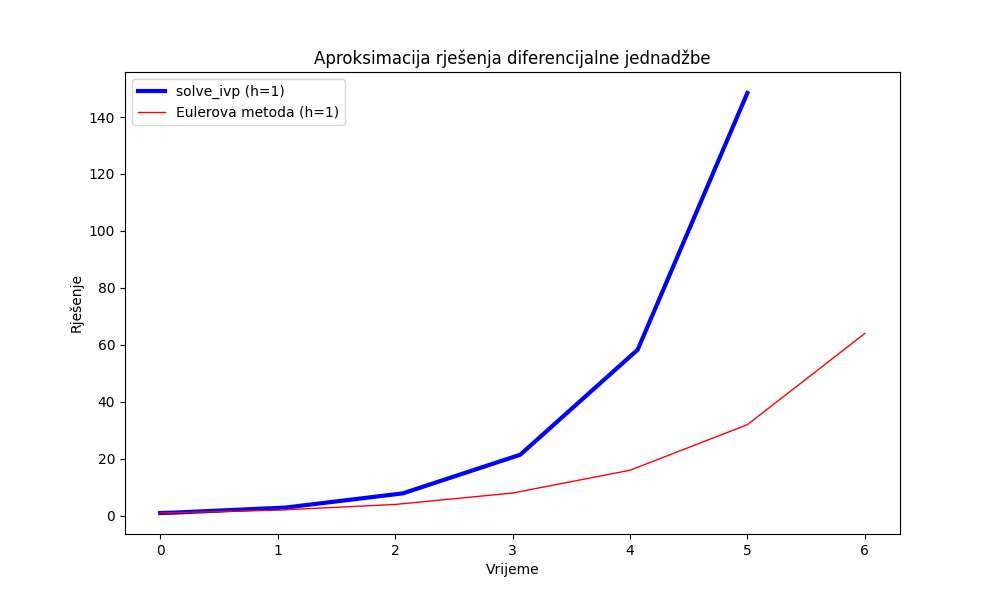
\includegraphics[width=0.5\textwidth]{slike/Figure_1.png}
        \caption{Inkrement: 1}
        \label{fig:Figure_1}
     \end{figure}
     \begin{figure}[htbp]
        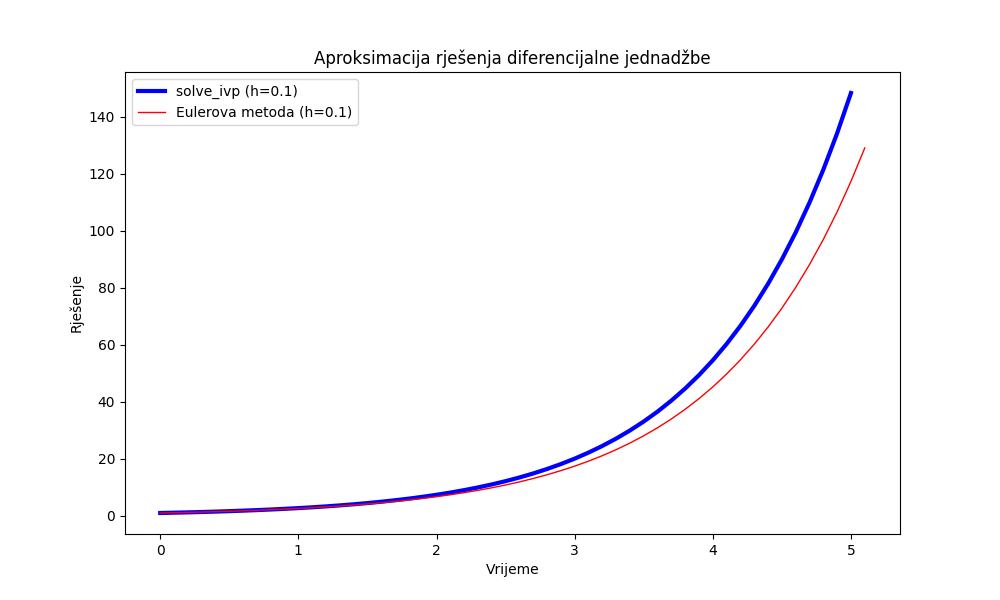
\includegraphics[width=0.5\textwidth]{slike/Figure_2.png}
        \caption{Inkrement: 0.1}
        \label{fig:Figure_2}
    \end{figure}
     \begin{figure}[htbp]
        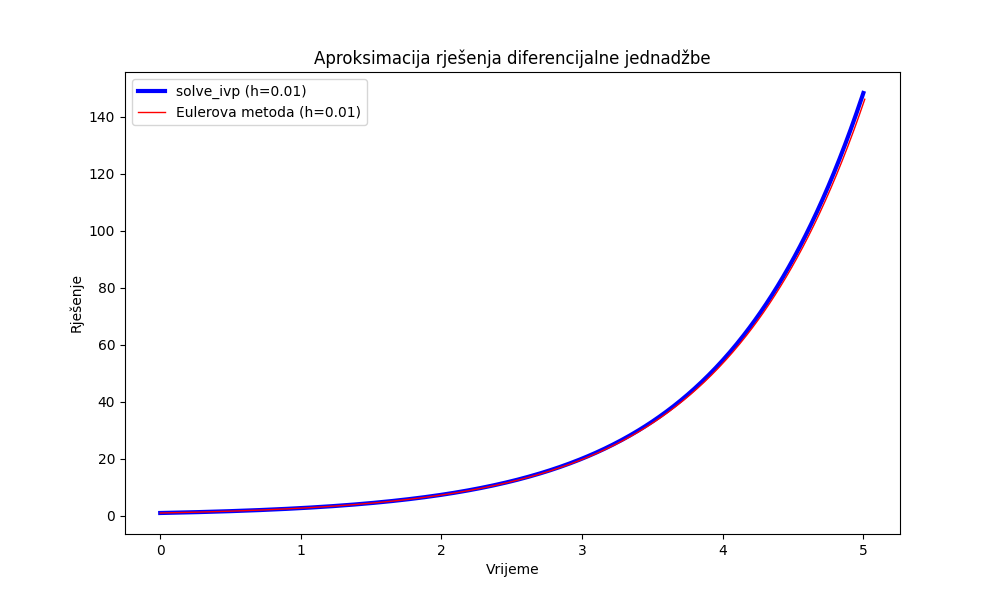
\includegraphics[width=0.5\textwidth]{slike/Figure_3.png}
        \caption{Inkrement: 0.01}
        \label{fig:Figure_3}
    \end{figure}
     \begin{figure}[htbp]
        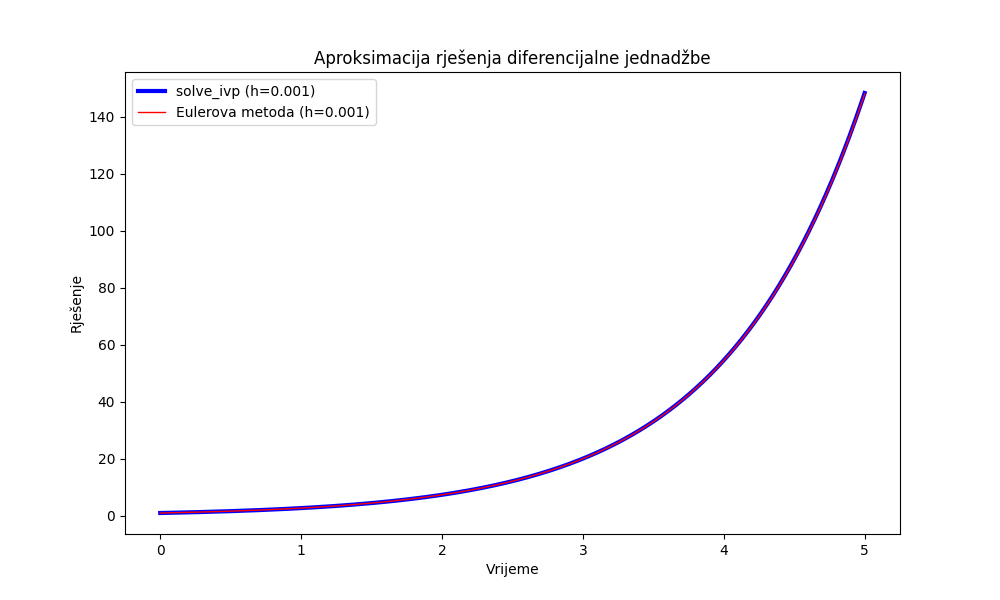
\includegraphics[width=0.5\textwidth]{slike/Figure_4.png}
        \caption{Inkrement: 0.001}
        \label{fig:Figure_4}
    \end{figure}
     \begin{figure}[htbp]
        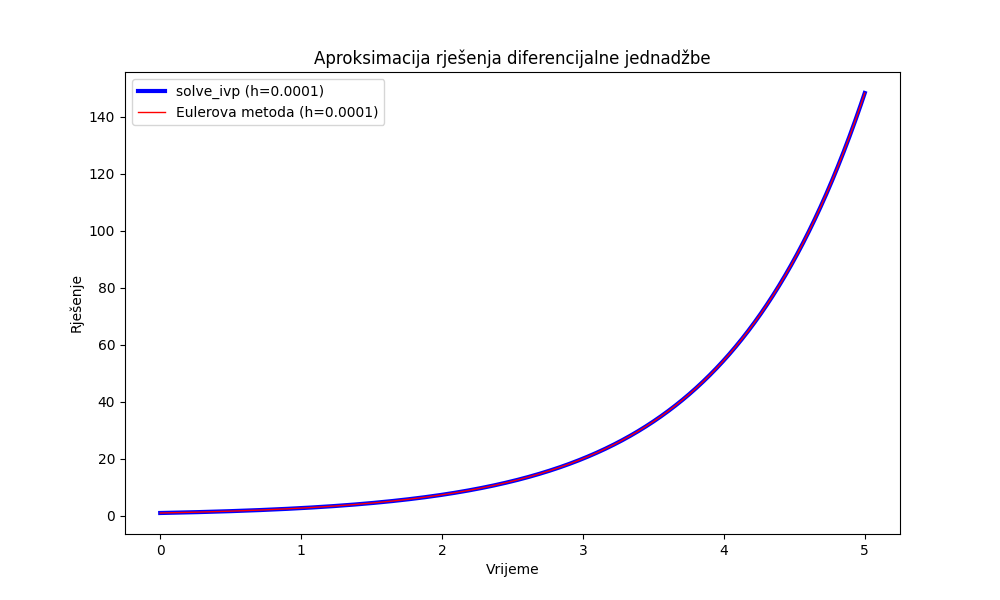
\includegraphics[width=0.5\textwidth]{slike/Figure_5.png}
        \caption{Inkrement: 0.0001}
        \label{fig:Figure_5}
    \end{figure}
     \begin{figure}[htbp]
        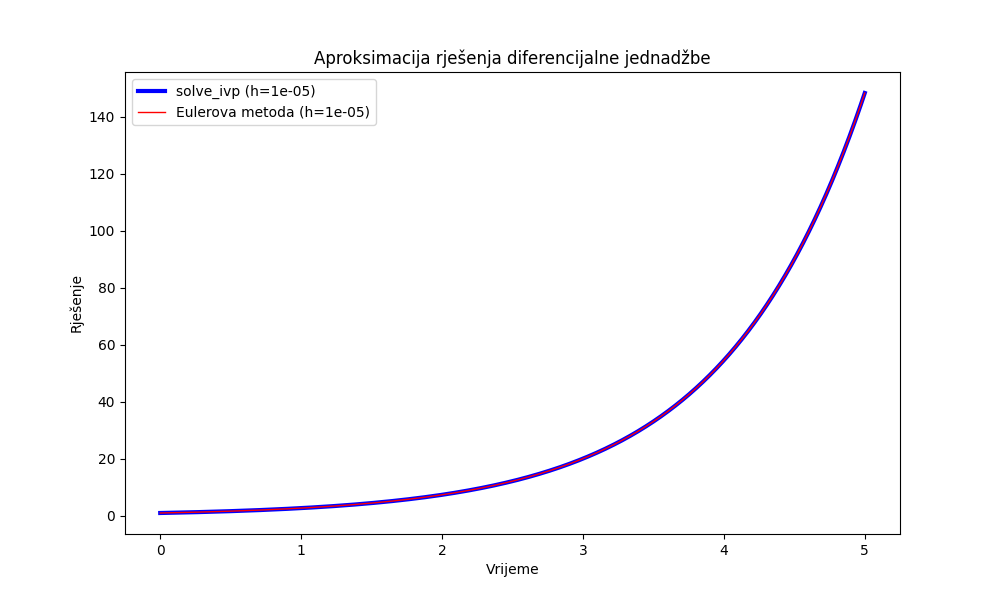
\includegraphics[width=0.5\textwidth]{slike/Figure_6.png}
        \caption{Inkrement: 0.00001}
        \label{fig:Figure_6}
    \end{figure}

\newpage
\section{Evaluacija}
\subsection{Pregled Literature:}
Proveli smo pregled literature kako bismo istražili najnovija postignuća u numeričkom rješavanju diferencijalnih jednadžbi s fokusom na Eulerovu metodu i paralelno računanje.
\subsection{Definiranje Varijabli i Parametara:}
Jasno smo definirali ključne varijable i parametre, uključujući postavke Eulerove metode, broj dretvi te inkrementalne korake, postavljajući temelj za eksperimentalni okvir.
\subsection{Implementacija u Pythonu:}
Koristili smo Python s NumPy, SciPy i MPI4py za implementaciju rješenja, uključujući funkcije za Eulerovu metodu, integraciju paralelnog računanja i skripte za testiranje.
\subsection{Eksperimentalno Testiranje:}
Provodili smo sustavno testiranje s pojedinačnim i višestrukim dretvama, varirajući inkrementalne korake. Rezultati su bilježeni radi usporedbe različitih pristupa.
\subsection{Analiza Rezultata:}
Analizirali smo rezultate kako bismo identificirali optimalni inkrement i procijenili učinkovitost pristupa rješavanju diferencijalnih jednadžbi. Prikazali smo vremenske performanse svakog testiranja kako bismo donijeli zaključke o prednostima i nedostacima svake varijante.\newline



\section{Zaključak}

\subsection{Budući Rad: Poboljšanja i Daljnje Istraživanje:}
U budućem istraživačkom radu, planiramo produbiti naša saznanja o paralelnom programiranju diferencijalnih jednadžbi, fokusirajući se na optimizaciju performansi i proširenje implementacije. Neki od ključnih aspekata koje planiramo istražiti uključuju:

\subsubsection{Unaprje\d{d}enje paralelnog računanja}
Analizirat \'cemo razli\v{c}ite strategije raspodjele poslova me\d{d}u dretvama, prou\v{c}avaju\'ci kako pode\v{s}avanje parametara paralelnog ra\v{c}unanja mo\v{z}e optimizirati brzinu izvo\d{d}enja. Razmatrat \'cemo i primjenu dodatnih tehnika paralelizacije, poput threadinga i multiprocessinga, kako bismo identificirali najefikasnije pristupe.

\subsubsection{Usporedba S Drugim Numeričkim Metodama}

Proširit ćemo našu analizu na usporedbu Eulerove metode s drugim numeričkim metodama za rješavanje diferencijalnih jednadžbi. Fokusirat ćemo se na Runge-Kutta metode, implicitne metode i druge tehnike kako bismo dobili sveobuhvatan uvid u performanse različitih pristupa.

\subsubsection{Optimizacija Implementacije u Pythonu}

Detaljnije ćemo istražiti efikasnost implementacije u programskom jeziku Python, razmatrajući ograničenja i prednosti ovog jezika u kontekstu znanstvenih izračuna. Planiramo predložiti optimizacije i prilagodbe kako bismo postigli što bolje performanse.

\subsubsection{Analiza Skalabilnosti i Robusnosti}

Provest ćemo dublju analizu skalabilnosti paralelnog algoritma, posebno promatrajući kako se povećanje broja dretvi odražava na ukupno vrijeme izvršavanja. Identificirat ćemo prepreke i ograničenja te razviti strategije za poboljšanje skalabilnosti i robustnosti algoritma.

\subsubsection{Primjena u Stvarnim Scenarijima}

Kako bismo validirali primjenjivost naših rezultata u stvarnim scenarijima, planiramo testirati algoritam na problemima iz stvarnog svijeta. Ovo uključuje složenije diferencijalne jednadžbe iz različitih znanstvenih disciplina, poput fizike, biologije ili inženjeringa.\newline

Kroz ove daljnje korake, očekujemo proširenje spoznaja o utjecaju paralelizacije na rješavanje diferencijalnih jednadžbi, s naglaskom na praksi, te pružanje smjernica za buduće istraživače i praktičare u području znanstvenog računanja.

\subsection{Literatura}

Link \cite{Stack} 
Link \cite{Pik}
Link \cite{Youtube1}
Link \cite{Youtube2}


\bibliographystyle{IEEEtran}
\bibliography{refs}

\end{document}
